\chapter{Exploration}\label{exploration}

This chapter presents the exploration phase of the design process.
Through an initial survey and a sequence of interviews, a whole range of
problems was explored before a single problem, scope, was put into
focus. By looking at solutions to conceptually similar problems and an
ideation phase, a series of concepts was sketched out.

\section{Survey \& Interviews}\label{survey-interviews}

To form a general understanding of how IDEs and some of their specific
features are used, an online survey targeted towards professional
developers was created. The survey ran in April 2014 over the course of
two weeks and yielded answers from 45 participants.

Besides general questions, e.g. which programming languages and IDEs the
participants used, it collected information about the usage of the
following IDE functionalities:

\begin{itemize}
\itemsep1pt\parskip0pt\parsep0pt
\item
  Navigation of code
\item
  Debugging
\item
  API and language documentation
\item
  Autocompletion
\item
  Project structure and scaffolding
\item
  Asynchronicity
\item
  Syntax Highlighting
\end{itemize}

For each of the areas the survey asked if and how the participants were
using them and—if appropriate—how their IDE was supporting them. The
survey instrumented multiple-choice questions with an additional „Other“
field for custom answers, as well as open-ended questions with a
free-form text field.

\subsection{Survey Results}\label{survey-results}

The survey participants listed 21 different programming languages they
are using on a regular basis, as well as experience in 19 different
development environments. The participants’ background is diverse,
although the major part seems to be working with web technologies (both
front-end and back-end).

About 76\% of the participants look up documentation mainly on the web,
only a small percentage uses the integration of documentation into IDEs.
However, nearly every participant (87\%) makes use of the IDE-provided
autocompletion feature, although most of them came up with ways to
improve it. Many comments are directed towards „smarter“, more
context-aware autocomplete suggestions, up to levels of artificial
intelligence. Some comments also mention a lack of performance and
subtlety.

Navigation within large code bases is done in many different ways, such
as presented before: file browsers, symbol browsers, file search or
content search. However, there does not seem to be a clear general
preference. For structuring code, most participants rely on
platform-given modularity, for example through packages and classes in
Java. In programming languages where project structures are not given,
developers use frameworks and design patterns to achieve a similar
structural consistency.

All participants value syntax highlighting, although for different
reasons. However, some offered suggestions on how highlighting of
certain code tokens could be used otherwise to reduce errors. Two
suggestions were targeted towards highlighting of \emph{similar}
identifiers in order to recognize typos. Others, however, intended to
focus on semantics instead of syntax; for example, indicating value
changes of the \emph{this} keyword in JavaScript, highlighting the
currently focused block of code, or colour-coding the relationship of
interdependent variables.

\subsection{Interview Results}\label{interview-results}

In succession to the survey, ten participants agreed to be interviewed,
seven of which the author conducted interviews with. The interviewees
are either currently working as full-time or part-time professional
developers or have been doing so in the past and are now in related
positions such as \emph{IT consultant}. Aside from that, their
backgrounds are diverse, ranging from part-time front-end developers
with a focus on design, over web application developers to low-level
audio specialists. They have experience with 12 different IDEs, using 15
programming languages on three different operating systems. Below is a
summary of interview results that are related to the thesis project.

Nearly all the interviewees stressed the importance of
\emph{performance} in any software development tool, especially in IDEs
and code editors. If a feature is too slow, reacts too slowly or slows
the overall IDE down, it is considered obtrusive and disturbing to the
development workflow. Especially the web developers praised lightweight
code editors, favouring them over the more heavyweight IDEs, but still
recognizing their drawbacks: lightweight editors are not as \emph{smart}
(see below).

Most of the interviewees also referred to their development tools of
choice in regards to the \emph{Unix philosophy}, which—according to Ken
Thompson—states that programs should „do one thing and do it well.“
\cite{raymond} This thought ultimately leads to modularily designed
systems, which was stressed in the interviews in different forms. Most
obvious is the ability to enable and disable features, as well as some
kind of plug-in management in general. Two interviewees also mentioned
\emph{modes}, although in different contexts. On the one hand, features
could run in different modes to provide help or stay out of they
developer’s way (\emph{beginner and expert modes}), on the other hand
modes could be used to get a different perspective on a program (e.g.
highlighting of different aspects in the code).

The interviewees expect their development environment to behave in a
\emph{smart} way; it should ideally know beforehand what the developers
need in terms of support in a given situation, and what code they are
about to write. On first look, and given the current landscape of IDEs
and text editors, this contradicts the desire for a lightweight, fast,
unopinionated development environment. To be smart, a development
environment must have knowledge about the programming language, the
libraries used, and about best practices. Some IDEs are tightly
integrated with their target programming platforms, for example
Microsoft Visual Studio with the .Net platform and Eclipse with the Java
platform. But these programs are generally not considered lightweight,
performant or unopinionated. \emph{Smartness} for lightweight
environments, however, can be achieved by combining it with the modular
approach of the Unix philosophy. If specialized programming language
tools can be loosely plugged into lightweight development environments,
smartness can be achieved in those environments as well. A good example
for this is given by the numerous \emph{Linter} plug-ins for editors
like Sublime Text (see section
\fullref{solutions-to-analogous-problems}) and projects like
CTags\footnote{See \url{http://ctags.sourceforge.net/}}.

The last relevant result of the interviews to be mentioned in this
section is a \emph{focus on code}. No matter the target platform and the
developer’s background, code is still in focus of the development
process nowadays, which makes the code editor the most important part of
any development environment. The term \emph{inline} describes activities
that happen within the text editor itself, for example syntax
highlighting. If development tools work inline, the developer does not
have to switch focus back and forth from the authoring process. However,
by putting additional information inline, there is a risk that the text
editor becomes too cluttered or visually busy, confusing and distracting
the developer. This is exemplified by pop-up windows that block a lot of
editor space or additional coloured text that makes colour-coding
ambiguous. Thus, programming tools that display information inline must
be carefully designed to be unobtrusive.

Four important characteristics for programming environments can be
extracted from the interviews: \emph{performance}, \emph{modularity},
\emph{smartness} and a \emph{focus on code}. Integrating these
characteristics is important for the usability and usefulness of
development environments, and thus for any tools that enhance them.

\subsection{Scope as a valid problem}\label{scope-as-a-valid-problem}

Through the conducted interviews and the survey, one can argue that
\emph{scope} is a promising and valid problem area to explore. Although
it was not referred to in the survey in any way, \emph{scope} was
mentioned independently by several of the survey participants and
interviewees in suggestions for the improvement of existing patterns and
tools. One of the interviewees introduced Crockford’s
\citeyear{crockford} approach of \emph{context colouring} (see below). A
similar approach was suggested in the survey in the context of editing.
Though not necessarily related to scope, the participant suggested to
highlight the current code block the cursor is placed in; this is
already done by some editors and IDEs, and is adapted in the concept
presented in this thesis as well. Another interviewee suggested to
indicate changes of the \emph{this} context in JavaScript, which is
closely related to scope, although being run-time specific.

The strongest alternative problem to possibly focus on was
\emph{asynchronicity} and the writing and debugging of asynchronous
code. After some research on the topic, I found the work of
\citeasnoun{lieber} to be quite substantial and possibly parallel to my
then-prospective work. Lieber implements \emph{Theseus}, an asynchronous
JavaScript debugger, and will discuss it from an Interaction Design
perspective in his forthcoming master’s thesis. This is why I did not
choose the topic of asynchronicity, but instead focused on the problem
of scope.

\section{Solutions to analogous problems}\label{similar}

The most ubiquitous visualization of program structure is probably
\emph{syntax highlighting} or \emph{syntax colouring}. This concept aims
to make the developer distinguish entities of the programming language
by showing them in different font types, weights, styles, or colours.
According to the survey results (see section
\fullref{survey-interviews}), syntax highlighting can help with a number
of different problems: recognizing errors and typos, distinguishing
language constructs from variables and values, and orienting through
specific visual patterns. Figure \ref{fig:syntaxhighlighting} shows
syntax highlighting in an HTML document; HTML elements are printed in
blue, whereas attributes are printed in purple, values in red, comments
in yellow, and content in black.

\begin{figure}[htbp]
\centering
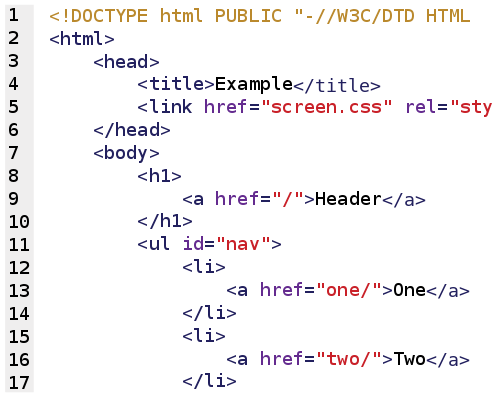
\includegraphics[keepaspectratio,width=0.75\textwidth]{img/syntax_highlighting.png}
\caption{Syntax highlighting in an HTML document}
\label{fig:syntaxhighlighting}
\end{figure}

In his talk „Monads and Gonads“, \citename{crockford} presents an
alternative to syntax highlighting which he calls „context colouring“
\citeyear{crockford}. Instead of using font styles and colours in order
to highlight different elements of the \emph{syntax}, he instead
highlights different \emph{scopes}. Figure \ref{fig:contexthighlighting}
illustrates this concept: The global scope is presented in white,
whereas nested scopes are marked green, yellow and blue, respectively.
In this concrete example, identifiers are always coloured in the colour
of the scope of \emph{where they were defined}. For example, the
appearance of \texttt{value} in the innermost scope is yellow, the
colour of the scope in which \texttt{value} was declared (as a function
parameter to the function \texttt{unit}).

\begin{figure}[htbp]
\centering
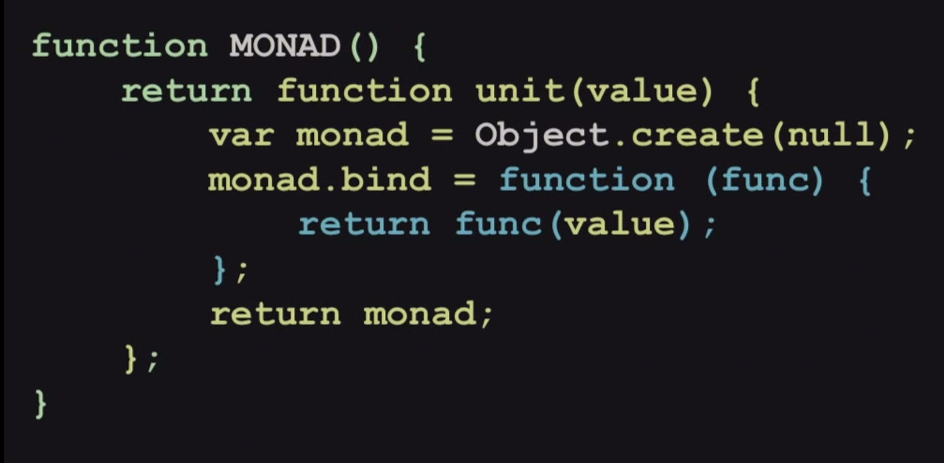
\includegraphics[keepaspectratio,width=0.75\textwidth]{img/context.png}
\caption{Context colouring in JavaScript, as proposed by Crockford (2013)}
\label{fig:contexthighlighting}
\end{figure}

\textbf{Theseus} is a JavaScript debugger built as a plug-in for the
Brackets IDE. It makes use of the code editor itself and shows
information inline, in the gutter and in a panel on the bottom of the
Brackets window (see Figure \ref{fig:theseus}). Theseus is mostly used
for asynchronous debugging, so the way those UI elements are used
corresponds to this purpose. For every function definition, Theseus
shows the number of times the function has been called in the gutter.
Functions that have never been called are marked with a grey background
in the source code. Additionally, the panel on the bottom shows
information about the function the cursor is positioned
in\footnote{It shows asynchronous call stacks, which are not of relevance to this thesis.}.

\begin{figure}[htbp]
\centering
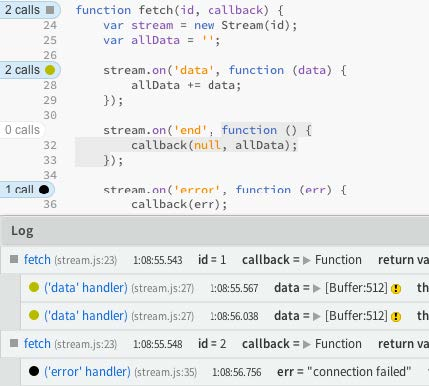
\includegraphics[keepaspectratio,width=0.5\textwidth]{img/theseus.jpg}
\caption{Theseus’ asynchronous JavaScript debugging (Lieber et al. 2014)}
\label{fig:theseus}
\end{figure}

\textbf{JSHint} is a so-called \emph{linting} tool, or \emph{linter},
for JavaScript: it detects bad programming practices (\emph{code
smells}) by checking JavaScript code against a set of rules, and
therefore tries to prevent common problems. Originally built as a
command-line tool and for online code checking, JSHint is implemented in
many IDEs through the respective plug-in systems. The \emph{Sublime
Linter} plug-in\footnote{See \url{http://www.sublimelinter.com/}} for
Sublime Text 3 implements JSHint (and other linting tools)
\emph{inline}: hints of bad code or inconsistent style are shown in the
text editor itself and are indicated in the gutter. If the cursor is on
top of problematic code, the respective hint is printed in the status
bar. \emph{Sublime Linter} behaves according to the characteristics
identified before: it is modular, as linters for different programming
languages can be plugged-in; it is lightweight and does not slow the
editor down; it focuses on code by displaying results inline without
cluttering the editor window; and it is smart to some extent, as it
allows the configuration of certain programming guidelines. The
prototype presented later in this thesis borrows many characteristics
and design decisions from linting tools such as this one. This is due to
the fact that both the problem of code smells and the problem of scope
can mostly be solved with static
analysis\footnote{Static analysis is the analysis of computer software that is performed without actually executing the program.}
and presented in a similar manner.

(Sublime Linter screenshot)

In terms of navigating and displaying tree structures in relation to the
actual source code, the \emph{Element Inspector} of \textbf{Chrome
Developer Tools} makes a good example (see Figure \ref{fig:devtools}).
The structure of \acs{html} is quite similar to that of scope, as it is
nested in the same way, which is why ideas can be taken from the
Developer Tools. They show the source code of the inspected website and
allows the user to select any \acs{html} element within. In the
remaining parts of the window, information relevant to the selected
element is shown.

\begin{figure}[htbp]
\centering
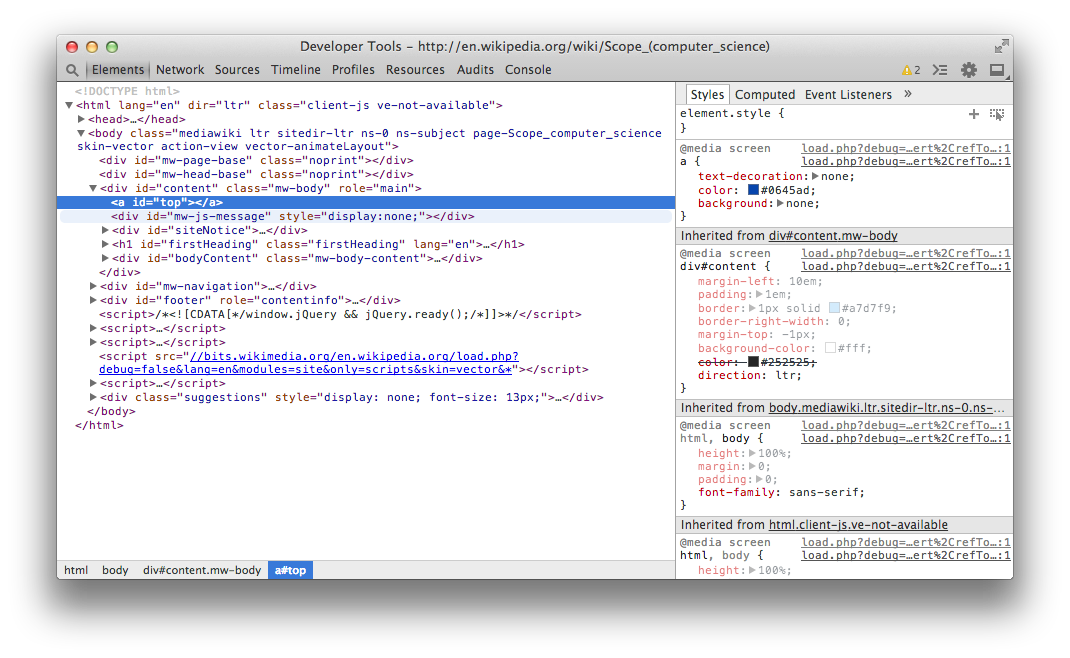
\includegraphics[keepaspectratio,width=\textwidth,height=0.75\textheight]{img/devtools.png}
\caption{Chrome DevTools with Element Inspector}
\label{fig:devtools}
\end{figure}

At the bottom of the window, a status bar shows the nesting of the
selected element: on the visual left (and logical top of the tree) is
the \texttt{html} element, inside it the \texttt{body}, then a
\texttt{div} and finally the selected \texttt{a} element. This status
bar can be used to navigate around the nested elements by clicking on
them. Clicking on the \texttt{body} element highlights it in the source
code as well, and shows different style information on the right-hand
side.

Placed to the right of the source code is a sidebar. Although it
contains a tabbed interface to browse different facets of the selected
element, the one that is relevant is the one in focus on the screenshot,
\emph{Style}. The way style (through \ac{css}) is applied to HTML
elements is similar to the way nested scope works: style that is defined
on the containing elements may influence the style of the selected
elements, which is why the relevant styles are listed in order of
precedence. The style rules that apply with the highest precedence are
listed on top, while the rules with the least precedence are listed on
the bottom. Style rules that are overriden by rules of higher precedence
are striked through to indicate that they do not apply anymore. This way
of visualizing and organizing information about nested structures is
further used in the following concept and design phases (see section
\ref{ideation} and chapter \ref{design}).

\section{Ideation}\label{ideation}

To support the ideation phase, existing \ac{ui} components used within
IDEs, as presented in chapter \ref{research}, were collected. Those
components were written down on post-it notes and used as seeds for
\emph{seeded brainstorming}: for each of the components, a set of
solutions should be developed that are similar, related to or based on
the respective component. Most of the ideas that came out of the
brainstorming session made use of multiple components, for example the
\emph{scope chain} which is described further down: it made use of a
status bar as well as the code editor.

Some ideas of the brainstorming phase made it into first sketches.
Depending on if the idea depended on actual source code, the sketching
took two different approaches. For ideas that involved code, it was
important to work with real, functioning code. Therefore, two JavaScript
applications were created to serve as examples:

\begin{itemize}
\itemsep1pt\parskip0pt\parsep0pt
\item
  A small web server application, that parses a markdown-formatted text
  file and renders it into an HTML template. The application runs on
  Node.js and represents a typical control flow for e.g. a blogging
  engine (i.e. content + template = site).
\item
  A client-side script (runs in a web browser) that fetches JSON data
  and presents them on a website, by the click of a button. This script
  represents typical client-side UI code, connecting a button event to a
  function and presenting the result in the UI.
\end{itemize}

The two applications were written in different styles: the server-side
application decouples its tasks by putting them into specific, named
functions (as far as it was seen appropriate) and therefore has a
relatively flat tree structure. The client-side application, however,
nests all function definitions inside each other, resulting in nearly
one function definition on each line, and far deeper indentation (in
other words, higher code complexity and deeply nested scope). A good
solution for this design problem should address both of the cases.

Printouts of the two JavaScript files served as a basis for ideation
that involved source code. However, for concept ideas that would mainly
work with other UI components, such as a sidebar, or such concept ideas
that would introduce new UI components, a blank notebook was used for
sketching.

\textbf{TODO: source code examples will be in the appendix and be
referenced here}

\begin{itemize}
\itemsep1pt\parskip0pt\parsep0pt
\item
  \emph{Scope Chain} - a breadcrumb view of the current scope chain,
  similar to that of a selector chain in an HTML editor (screenshot!).
  The scope at the position of the cursor would be shown in a status
  bar. By hovering over a scope level, the corresponding source code
  would be highlighted in the source editor.
\item
  \emph{Scope Graph} - similar to a class browser, the scope graph would
  represent a tree view of the application’s scopes. This could be
  implemented as a sidebar or panel.
\item
  \emph{Scope Colouring} - similarly suggested by Crockford
  \citeyear{crockford}, the source code can be coloured in depending on
  its scope level. Crockfords variation is meant to replace syntax
  highlighting; one could, as well, complement syntax highlighting by
  colouring in the background (as e.g. Theseus does), e.g. in shades of
  grey.
\item
  \emph{Inspect Scope} - comparable to DevTools’ \emph{Inspect Element}
  function, the user can right-click into the source code and choose
  \emph{Inspect Scope}, which opens a panel that shows global variables,
  current local variables as well as the value of \texttt{this}.
\item
  \emph{Gutter Scope} - any change of scope is indicated in the code
  editor’s gutter (similar to JSHint).
\item
  \emph{Quick Inspect} - similar to Brackets’ \emph{Quick Edit} feature,
  the value of \texttt{this} could be inspected inline. Debugger stuff,
  as \emph{this} is run-time.
\end{itemize}

\textbf{TODO: more detail, and scans of relevant sketches (not! all of
them)}

\textbf{TODO: Chosen solution is combination of scope chain, scope
colouring and inspect scope}
